\documentclass[12pt, a4paper, twocolumn]{article}

%%%%%%%%%%%%%%%%%%%%%%%%%%%%%%%%%%%%%%%%%
%  THIS IS struct.tex to define the structure of the document 
%%%%%%%%%%%%%%%%%%%%%%%%%%%%%%%%%%%%%%%%%

%----------------------------------------------------------------------------------------
%	PACKAGES AND OTHER DOCUMENT CONFIGURATIONS
%----------------------------------------------------------------------------------------

\usepackage[english]{babel} % English language hyphenation

\usepackage{microtype} % Better typography

\usepackage{amsmath,amsfonts,amsthm} % Math packages for equations

\usepackage[svgnames]{xcolor} % Enabling colors by their 'svgnames'

\usepackage[hang, small, labelfont=bf, up, textfont=it]{caption} % Custom captions under/above tables and figures

\usepackage{booktabs} % Horizontal rules in tables

\usepackage{lastpage} % Used to determine the number of pages in the document (for "Page X of Total")

\usepackage{graphicx} % Required for adding images

\usepackage{enumitem} % Required for customising lists
\setlist{noitemsep} % Remove spacing between bullet/numbered list elements

\usepackage{sectsty} % Enables custom section titles
\allsectionsfont{\usefont{OT1}{phv}{b}{n}} % Change the font of all section commands (Helvetica)

\usepackage[hidelinks]{hyperref} 

% removing the red rectangle around section names in table of content


%----------------------------------------------------------------------------------------
%	MARGINS AND SPACING
%----------------------------------------------------------------------------------------

\usepackage{geometry} % Required for adjusting page dimensions

\geometry{
	top=1cm, % Top margin
	bottom=1.5cm, % Bottom margin
	left=1.5cm, % Left margin
	right=1.5cm, % Right margin
	includehead, % Include space for a header
	includefoot, % Include space for a footer
	%showframe, % Uncomment to show how the type block is set on the page
}

\setlength{\columnsep}{7mm} % Column separation width

%----------------------------------------------------------------------------------------
%	FONTS
%----------------------------------------------------------------------------------------

\usepackage[T1]{fontenc} % Output font encoding for international characters
\usepackage[utf8]{inputenc} % Required for inputting international characters
% \usepackage{fontspec}

% % Set the font to Times New Roman
% \setmainfont{Times New Roman}

% \usepackage{XCharter} % Use the XCharter font

% \usepackage{fontspec}
% \setmainfont{Arial}

%----------------------------------------------------------------------------------------
%	HEADERS AND FOOTERS
%----------------------------------------------------------------------------------------

\usepackage{fancyhdr} % Needed to define custom headers/footers
\pagestyle{fancy} % Enables the custom headers/footers

\renewcommand{\headrulewidth}{0.0pt} % No header rule
\renewcommand{\footrulewidth}{0.4pt} % Thin footer rule

\renewcommand{\sectionmark}[1]{\markboth{#1}{}} % Removes the section number from the header when \leftmark is used

%\nouppercase\leftmark % Add this to one of the lines below if you want a section title in the header/footer

% Headers
\lhead{} % Left header
\chead{\textit{\thetitle}} % Center header - currently printing the article title
\rhead{} % Right header

% Footers
\lfoot{} % Left footer
\cfoot{} % Center footer
\rfoot{\footnotesize Page~\thepage\ of \pageref{LastPage}} % Right footer, "Page 1 of 2"

\fancypagestyle{firstpage}{ % Page style for the first page with the title
	\fancyhf{}
	\renewcommand{\footrulewidth}{0pt} % Suppress footer rule
}

%----------------------------------------------------------------------------------------
%	TITLE SECTION
%----------------------------------------------------------------------------------------

\newcommand{\authorstyle}[1]{{\large\usefont{OT1}{phv}{b}{n}\color{DarkRed}#1}} % Authors style (Helvetica)

\newcommand{\institution}[1]{{\footnotesize\usefont{OT1}{phv}{m}{sl}\color{Black}#1}} % Institutions style (Helvetica)

\usepackage{titling} % Allows custom title configuration

\newcommand{\HorRule}{\color{DarkGoldenrod}\rule{\linewidth}{5pt}} % Defines the gold horizontal rule around the title

\pretitle{
	
	\vspace{-30pt} % Move the entire title section up
	\HorRule\vspace{10pt} % Horizontal rule before the title
	\fontsize{40}{48}\usefont{OT1}{phv}{b}{n}\selectfont % Helvetica
	\color{DarkRed} % Text colour for the title and author(s)
}

\posttitle{\par\vskip 30pt} % Whitespace under the title

\preauthor{\hspace*{\fill} \textbf{Group:K} \\
			\hspace*{\fill} Pandit Siddhesh Ashok,\\
		   \hspace*{\fill} Sujay Hansda,\\
		   \hspace*{\fill} Tarushri N S,\\
		   \hspace*{\fill} Yogendra Singh Laikara} % Author style (Helvetica)

\postauthor{ % Anything that will appear after \author is printed
	\vspace{10pt} % Space before the rule
	\par\HorRule % Horizontal rule after the title
	\vspace{20pt} % Space after the title section
	\begin{center}
		\vspace*{40pt}
		\institution{Indian Institute Of Science, Bengaluru}
	\end{center} % Institution
}

%----------------------------------------------------------------------------------------
%	ABSTRACT
%----------------------------------------------------------------------------------------
% 
% \usepackage{lettrine} % Package to accentuate the first letter of the text (lettrine)
% \usepackage{fix-cm}	% Fixes the height of the lettrine

% \newcommand{\initial}[1]{ % Defines the command and style for the lettrine
% 	\lettrine[lines=3,findent=4pt,nindent=0pt]{% Lettrine takes up 3 lines, the text to the right of it is indented 4pt and further indenting of lines 2+ is stopped
% 		\color{DarkGoldenrod}% Lettrine colour
% % 		{#1}% The letter
% 	}{}%
% }

% \usepackage{xstring} % Required for string manipulation

% \newcommand{\lettrineabstract}[1]{
% 	\StrLeft{#1}{1}[\firstletter] % Capture the first letter of the abstract for the lettrine
% 	\initial{\firstletter}\textbf{\StrGobbleLeft{#1}{1}} % Print the abstract with the first letter as a lettrine and the rest in bold
% }

%----------------------------------------------------------------------------------------
%	BIBLIOGRAPHY
%----------------------------------------------------------------------------------------

\usepackage[backend=bibtex,style=authoryear,natbib=true]{biblatex} % Use the bibtex backend with the authoryear citation style (which resembles APA)

\addbibresource{example.bib} % The filename of the bibliography

\usepackage[autostyle=true]{csquotes} % Required to generate language-dependent quotes in the bibliography

\usepackage{lipsum}

\title{\textbf{Coherent Imaging\\}} % The article title
\author{} % Author
\date{} % Add a date here if you would like one to appear underneath the title block, use \today for the current date, leave empty for no date

%----------------------------------------------------------------------------------------
\begin{document}
\begin{titlepage}

	\maketitle % Print the title
	\vspace*{10cm}
	
\end{titlepage}
\thispagestyle{firstpage}
\hrule
\tableofcontents
\vspace*{20pt}
\hrule
% \pagebreaks
\section{Introduction}
\subsection{What is coherence in imaging?}
Coherence is a property of light that describes the degree of correlation between the phases of different light waves. In imaging, coherence plays a crucial role in determining the quality and resolution of the captured images. Coherent light sources, such as lasers, produce light waves with a fixed phase relationship, allowing for the interference of light waves to create high-resolution images. Incoherent light sources, on the other hand, produce light waves with random phase relationships, resulting in lower-quality images with reduced resolution.
\textbf{coherence time}
for example we have the displacement equation $ E = A\cos(\omega t + \phi) $, where $\phi$ is the phase of the wave.  which states that at any value of x the displacement is sinusioidal with time. But Experimentally we can see that the light is not always coherent. The light is coherent only for a certain time period. This time period is called the \textbf{coherence time} of the light, denoted by $\tau_c$. Basically coherence time is the time for which the phase of the light remains constant. It is inversly proportional to the bandwidth of the light, i.e E will be sinusioidal for for time $\tau_c$. And $$L = \text{coherence length} = c\tau_c$$.
\par
Coherent imaging is a technique used in various fields, such as microscopy and holography, to obtain high-resolution images of objects. It relies on the interference of coherent EM waves to capture both the amplitude and phase information of the object being imaged.

One of the key advantages of coherent imaging is its ability to achieve diffraction-limited resolution, surpassing the limitations of traditional imaging techniques. By utilizing the wave nature of light, coherent imaging can reveal fine details and structures that are otherwise invisible.

In coherent imaging, a coherent source, such as a laser, is used to illuminate the object. The light waves scattered by the object are then combined with a reference wave to create an interference pattern. This interference pattern contains the information about the object's spatial frequencies and phase shifts.

To capture the interference pattern, various detection methods can be employed, including holography, interferometry, and digital image processing techniques. These methods allow for the reconstruction of the object's image with high fidelity.

Coherent imaging finds applications in a wide range of fields, including medical imaging, materials science, and non-destructive testing. It enables researchers and practitioners to study the intricate details of biological samples, analyze the properties of materials, and inspect the integrity of structures.

In conclusion, coherent imaging is a powerful technique that revolutionizes the way we capture and analyze images. Its ability to preserve both amplitude and phase information opens up new possibilities in imaging and paves the way for advancements in various scientific and technological domains.



\section{Types of Coherent Imaging}
	\begin{itemize}
		\item \textbf{Holography:} Holography is a technique that captures both the amplitude and phase information of an object by recording the interference pattern between the object wave and a reference wave. The hologram can then be reconstructed to produce a three-dimensional image of the object.
		\item \textbf{CDI:} Coherent Diffraction Imaging (CDI) is a method that uses the diffraction pattern of an object to reconstruct its image. By analyzing the diffraction pattern, can recover the object's amplitude and phase information without the need for lenses or other optical elements.
		\item \textbf{Interferometry:} Interferometry is a technique that combines two or more coherent light waves to create an interference pattern. By analyzing the interference pattern, interferometry can reveal the phase shifts and spatial frequencies of the object being imaged.
		\item \textbf{Digital Holography:} Digital holography is a method that captures holograms using digital sensors, such as CCD or CMOS cameras. By recording the interference pattern digitally, digital holography enables real-time reconstruction and analysis of holographic images.
		\item \textbf{Phase Contrast Imaging:} Phase contrast imaging is a technique that enhances the visibility of phase variations in transparent samples. By converting phase shifts into intensity variations, phase contrast imaging can reveal fine details and structures that are otherwise invisible.
		\item \textbf{optical coherence tomography:} Optical Coherence Tomography (OCT) is a non-invasive imaging technique that uses low-coherence interferometry to capture cross-sectional images of biological tissues. By measuring the echo time delay of light waves, OCT can create high-resolution images of tissue structures.
	\end{itemize}
	
	Here we are going to discuss the coherent diffractive imaging (CDI) technique in detail.
\section{Coherent Diffractive Imaging (CDI)}
	we can devide CDI into five main groups:
	\begin{itemize}
		\item \textbf{CDI in plane wave approximation:} Presented for first time[1].The coherent plane wave incident on illuminated sample we can record the diffraction pattern in far-field zone. The object is reconstructed by using the diffraction pattern.
		\item \textbf{CDI in Bragg geometry:} This method is used to study the crystal structure of samples. 
		\item \textbf{X-ray ptychography:} This method is used to study linear sizes of samples exceed the transverse sizes of incident X-ray beam. the latter is formed using pinhole and and focusing coherent X-ray beam.This implies scaning the sample over 2D extended objected, with simultaneous recording of diffraction patterns from partially overlapping regions of the sample.
		\item \textbf{Fresnel approximation:} A sample is placed before focal plane of Fresnel zone plane after which 2D diffraction data recorded.
		\item \textbf{CDI in TIR:} sample is placed on the surface of substrate and geometry is fixed in closed to total internal reflection (TIR) condition. 
	
	\end{itemize}
	CDI methods make it possible to study the chemical, elemental, structural and magnetic properties of nanoscale objects. These methods is used in various fields such as biology, medicine, materials science, and nanotechnology.
	% \newpage
	% \pagebreak
	% adding plane_wave_approximation.png ptichography.png bragg_geometry.png fresnel_approximation.png TIR.png
% 	\begin{figure*}[h]
% 		\begin{minipage}{0.5\textwidth}
% 			\centering
% 			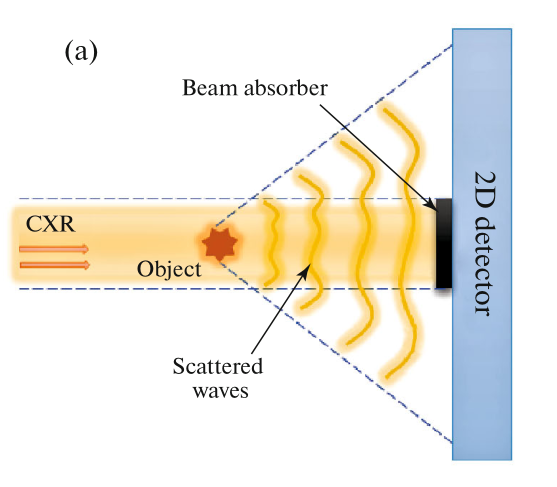
\includegraphics[width=0.48\textwidth]{plane_wave_approximation.png}
% 			\caption{CDI in plane wave approximation}
% 		\end{minipage}%
% 		\begin{minipage}{0.5\textwidth}
% 			\centering
% 			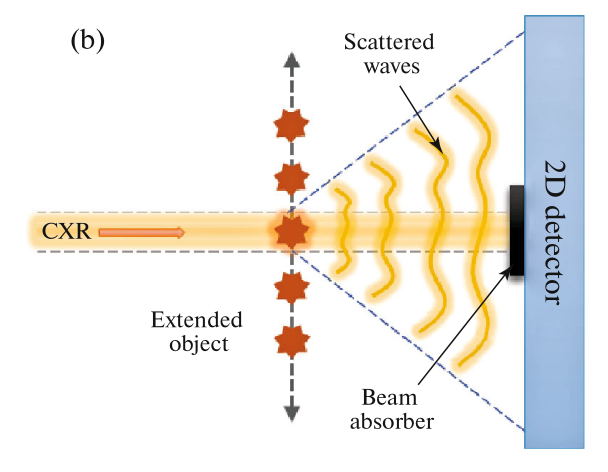
\includegraphics[width=0.48\textwidth]{ptychography.png}
% 			\caption{X-ray ptychography}
% 		\end{minipage}
	
% 		\begin{minipage}{0.5\textwidth}
% 			\centering
% 			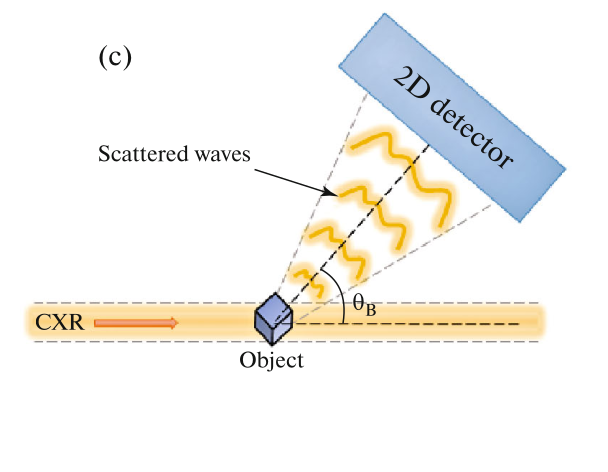
\includegraphics[width=0.48\textwidth]{braggs-geometryy.png}
% 			\caption{CDI in Bragg geometry}
% 		\end{minipage}%
% 		\begin{minipage}{0.5\textwidth}
% 			\centering
% 			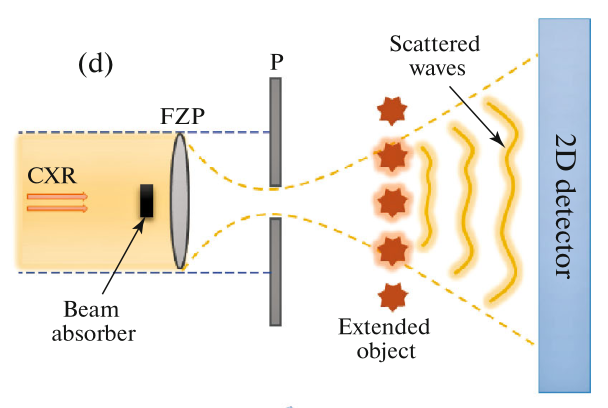
\includegraphics[width=0.48\textwidth]{Fresnel approximation.png}
% 			\caption{Fresnel approximation}
% 		\end{minipage}
	
% 		\centering
% 		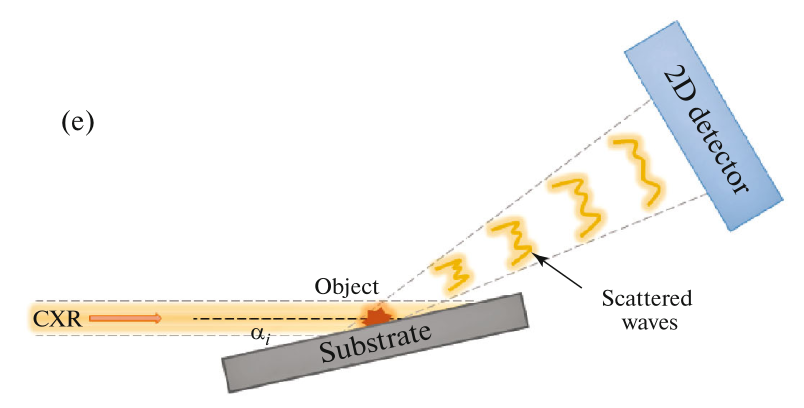
\includegraphics[width=0.5\textwidth]{TER_geometry.png}
% 		\caption{CDI in TIR}
% 	\end{figure*}
% \hrule
% % \pag
\section{Basic Applications of Coherent Imaging}
	\begin{itemize}
		\item \textbf{Biological Imaging:} Coherent imaging is widely used in biological imaging to study the structure and function of biological samples. By capturing both the amplitude and phase information of biological tissues, coherent imaging can reveal fine details and structures that are otherwise invisible.
		\item \textbf{Materials Science:} Coherent imaging plays a crucial role in materials science by enabling researchers to analyze the properties and structures of materials. By studying the diffraction patterns of materials, coherent imaging can provide valuable insights into their composition, crystal structure, and defects.
		\item \textbf{Non-Destructive Testing:} Coherent imaging is used in non-destructive testing to inspect the integrity of structures and components. By analyzing the interference patterns of light waves, coherent imaging can detect defects, cracks, and other imperfections in materials without causing damage.
		\item \textbf{Medical Imaging:} Coherent imaging is employed in medical imaging techniques, such as optical coherence tomography (OCT), to capture high-resolution images of biological tissues. By measuring the echo time delay of light waves, OCT can create cross-sectional images of tissues with micrometer-scale resolution.
		\item \textbf{Nanotechnology:} Coherent imaging is used in nanotechnology to study the properties and behavior of nanoscale objects. By analyzing the diffraction patterns of nanoparticles and nanostructures, coherent imaging can provide valuable insights into their chemical, structural, and magnetic properties.
	\end{itemize}

	In this we are going to see some application and research on CXDI:\par
	\vspace*{10pt}
\begin{minipage}{0.5\textwidth}
	

	\fbox{
	\begin{minipage}{0.8\textwidth}
	\begin{itemize}
		\item 3D imaging of dislocations in a nanoparticle at atomic resolution.
		\item Three-dimensional imaging of dislocation propagation during crystal growth and dissolution.
		\item Coherent diffraction imaging of nanoscale strain evolution in a single crystal under high pressure.
		\item Three-dimensional coherent X-ray diffraction imaging of a whole, frozen-hydrated cell
	\end{itemize}
	\end{minipage}
	}
\end{minipage}

\subsection{3D imaging of dislocations in a nanoparticle at atomic resolution}
The study explores the 3D imaging of dislocations in a Pt nanoparticle at atomic resolution using electron tomography. Dislocations are crucial for understanding material properties and can be visualized at the atomic level using methods like transmission electron microscopy (TEM). However, traditional methods provide only 2D projections of 3D objects, making X-ray topography and other methods limited in resolution.\par
The researchers successfully imaged nearly all the atoms in a multiply twinned Pt nanoparticle using this approach. They observed atomic steps at 3D twin boundaries and the 3D core structure of edge and screw dislocations at atomic resolution. These dislocations and atomic steps at the twin boundaries, which appear to be stress relief mechanisms, were not visible in conventional 2D projections.\par
The method involves combining annular dark field scanning TEM with specific tomographic techniques to achieve high-resolution 3D imaging. Pt nanoparticles were synthesized using peptide sequences in aqueous solution and supported on 5 nm thick silicon nitride membranes. To stabilize the nanoparticles under a scanning transmission electron microscopy (STEM) beam, a thin Carbon layer was deposited on the Pt nanoparticles and electron energy was kept below the knock-on radiation damage threshold of Pt.

A 3D reconstruction of the nanoparticle was obtained using the EST method, but 3D dislocations could not be identified in the raw 3D reconstruction at atomic resolution. To enhance the signal-to-noise ratio (SNR), a 3D Fourier filtering method was developed to identify all measurable 3D Bragg peaks and the 3D distribution around each peak.\par
In summary, this research showcases a significant advancement in imaging 3D dislocations in materials at atomic resolution, providing new insights into the behaviour of materials at the atomic level. The methods and findings presented in this study have implications for materials science, nanoscience, solid-state physics, and chemistry, and pave the way for further advances in imaging the 3D local structure of materials at high resolution.\\
Some example figures are shown below:\par
% add image 3d_di.png
\begin{figure}[h]
	% \centering
	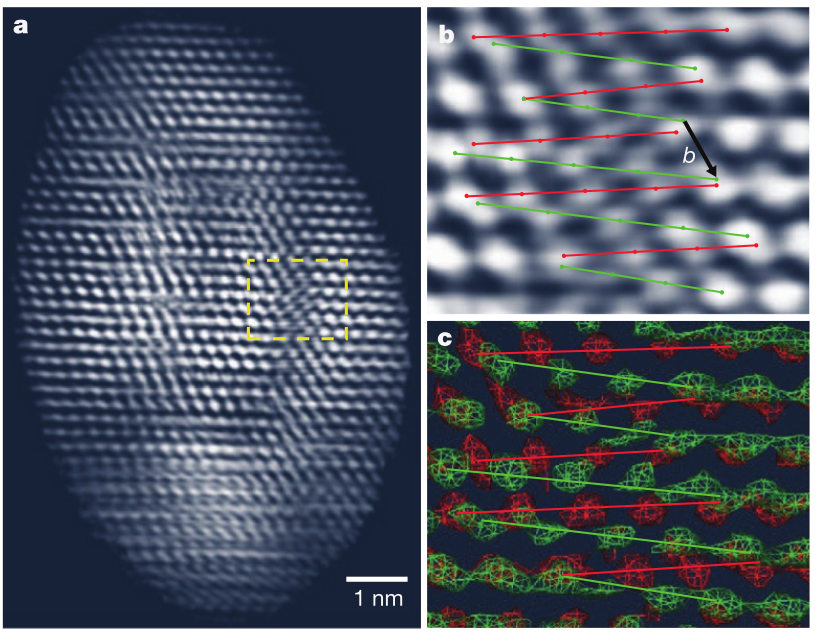
\includegraphics[width=0.35\textwidth]{3d_di.png}
	\caption{Observation of the 3D core structure of a screw dislocation at	atomic resolution.
	}
\end{figure}
\textbf{figure 1:} Volume renderings of a $5.3 $thick slice (two atomic
layers) in the [111] plane, tilted to the [011] direction
to visualize the zigzag pattern, a characteristic feature of a screw dislocation.b, Enlarged view of a screw dislocation showing the zigzag pattern. c, Surface
renderings of the screw dislocation where the atoms represented by green dots are in the top layer and those by red dots are in the bottom layer. The zigzag pattern is more clearly visualized, the Burgers vector (b) of the screw dislocation was determined to be $\frac{1}{2}[011]$, and the width of the screw dislocation was estimated to be ,8.9 Å.
% adding image 3d_di2.printing
\par

\begin{figure}[h]
	% \centering
	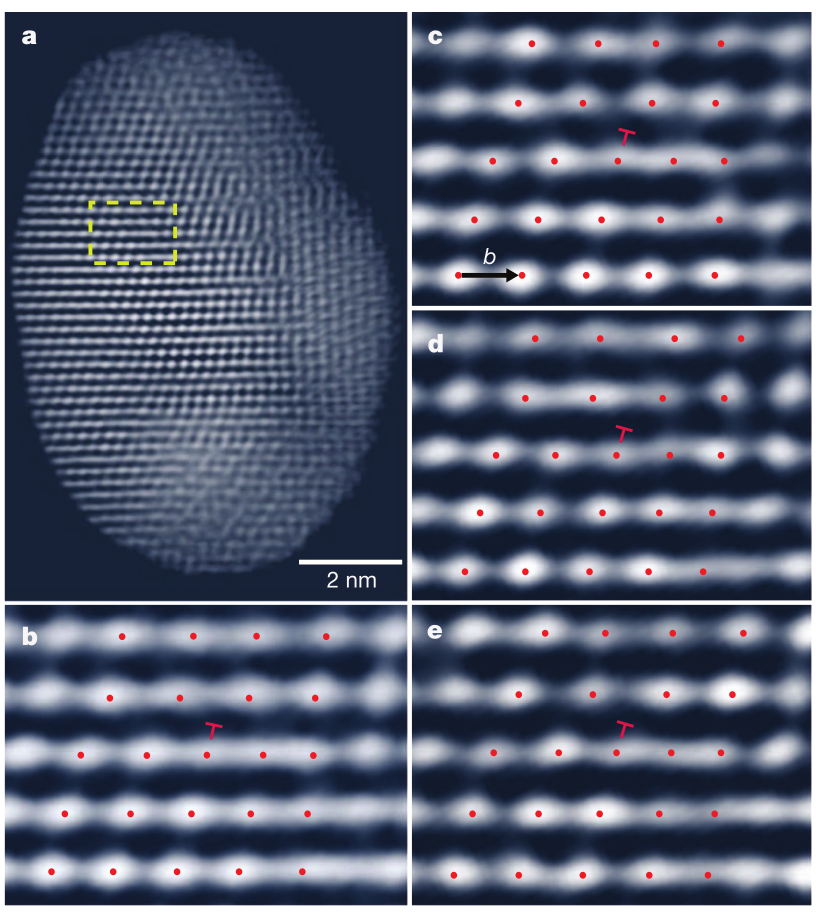
\includegraphics[width=0.35\textwidth]{3d_di2.png}
	\caption{Observation of the 3D core structure of an edge dislocation at	atomic resolution.
}
\end{figure}
\textbf{figure 2:} \textbf{a}, A $7.9 angstrom $thick internal slice of the nanoparticle. The lattice structure on the left and at the bottom parts of the slice is not well defined,
mainly because this decahedral multiply twinned nanoparticle consists of five
grains with different orientations. \textbf{b}, An enlarged view of an edge dislocation in \textbf{a} where red dots represent the position of the atoms. \textbf{c, d} and \textbf{e}, $2.6 angstrom$thickatomic layers sectioning through the slice of b. The three consecutive atomiclayers indicate the dislocation line is in the direction of $\frac{1}{2}$[101]. The Burgers vector(b) of the edge dislocation was determined to be $\frac{1}{2}[101]$.

\subsection{Three-dimensional imaging of dislocation propagation during crystal growth and dissolution}
The study delves into the three-dimensional imaging of dislocation propagation during crystal growth and dissolution, aiming to comprehend the mechanisms influencing material properties. Dislocations, being defects within the crystal lattice, significantly impact mechanical, electrical, and optical traits. Various imaging techniques, such as X-ray computed tomography, electron tomography, and optical microscopy, facilitate the visualization of dislocations in three dimensions. These methods entail capturing images of the crystal from different angles and depths, reconstructing them into a 3D volume, and employing image processing to identify dislocations. Researchers interpret these findings to grasp dislocation propagation during crystal growth or dissolution, aiding in optimizing manufacturing processes and enhancing material properties.\par

Moreover, the research paper introduces a novel application of Bragg coherent diffractive imaging (BCDI) to scrutinize dislocation behavior within individual calcite crystals during growth and dissolution. Utilizing BCDI, the study seeks to provide a comprehensive understanding of how crystallographic defects, particularly screw dislocations, influence crystal growth and dissolution mechanisms. The focus on calcite crystals serves as a model system to explore the intricate relationship between dislocations and crystal morphology. Such investigations deepen our understanding of crystal growth processes and offer insights into controlling and optimizing material synthesis techniques for improved outcomes.
% adding image 3d_imaging_growth.png
\begin{figure}[h]
	% \centering
	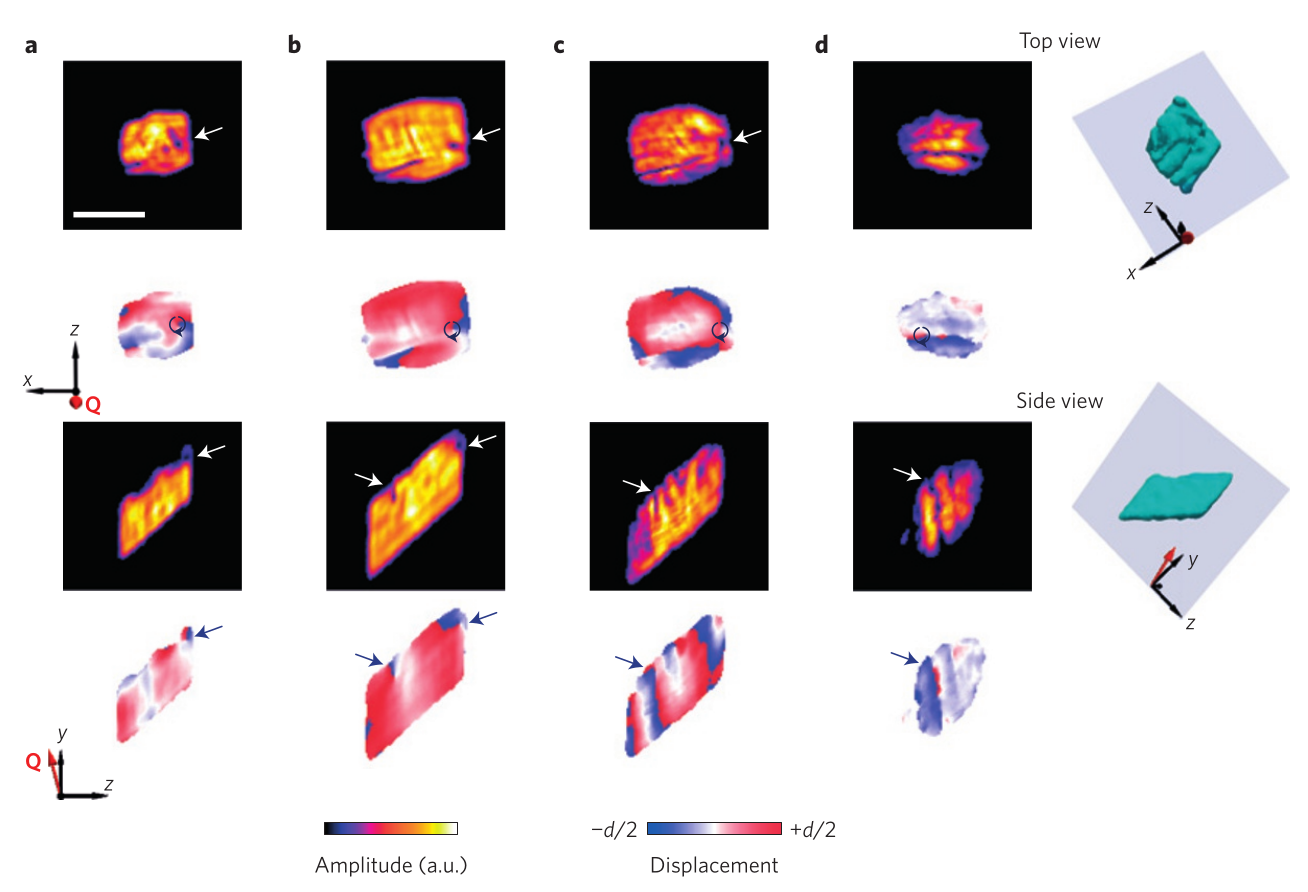
\includegraphics[width=0.4\textwidth]{3d_imaging_crystal_growth.png}
	\caption{Slices showing the electron density and projected displacement during growth and dissolution.
			}
\end{figure}
\par \textbf{figure 3:}\textbf{a–d}, Crystal in the initial state (\textbf{a}), and after growth (\textbf{b}) and repetitive dissolution steps (\textbf{c,d}) for two viewing directions (top view) and (side view). The amplitude is shown in the top rows (black background) with the  dislocations highlighted by white arrows featuring a low-amplitude core. The phase presented in the bottom rows also showsselected dislocations highlighted by the dark blue arrows. Particularly evident is the spiral phase (displacement) that is characteristic of a screw dislocation. The iso-surface to the right shows the location of the cut planes. The scale bar is 1 µm.
\subsection{Coherent diffraction imaging of nanoscale strain evolution in a single crystal under high pressure}
\par The study explores the three-dimensional strain distribution of a 400 nm gold single crystal during compression within a diamond-anvil cell using the mutual coherent function method. The aim is to understand the evolution of morphology and internal strain under high pressure, its implications for physical properties, structural stability, phase transition, and deformation mechanism of materials. The research introduces the Bragg coherent X-ray diffraction imaging (CXDI) technique as a promising tool to probe the internal strain distribution of individual nanometre-sized single crystals. The experimental setup uses a large opening panoramic diamond-anvil cell to compress the gold crystal, and X-ray sensitive charge-coupled devices collect far-field diffraction patterns. The results show 3D reconstructions of morphology and phase under pressures, showing changes in crystal shape, phase shift, and strain distribution with increasing pressure. The findings have potential implications for fundamental physics and applied sciences, as well as new approaches in high-pressure nanotechnology development. Overall, the study demonstrates the high resolution of Bragg CXDI for studying morphology and internal strain evolution under high pressure, providing a promising approach for in-situ nanotechnology development under high pressures.
% adding image expsetup.png
\begin{figure}[h]
	% \centering
	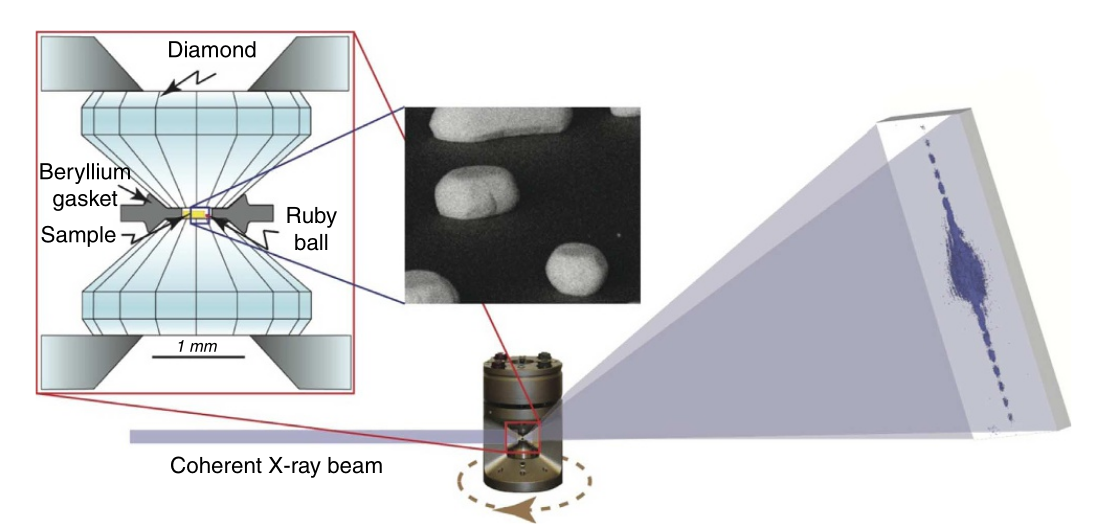
\includegraphics[width=0.5\textwidth]{expsetup.png}
	\caption{Experimental setup for coherent X-ray diffraction imaging of a single crystal under high pressure.
	}
\end{figure}

\subsection{Three-dimensional coherent X-ray diffraction imaging of a whole, frozen-hydrated cell}
the study demonstrates the efficacy of cryogenic coherent diffraction imaging (cryo CDI) in elucidating the three-dimensional structure of whole, frozen-hydrated cells with unprecedented detail and resolution. By utilizing 8 keV X-rays and employing advanced techniques to alleviate radiation damage, the researchers successfully overcame previous limitations associated with structural imaging at high spatial resolutions.

The experimental setup involved the precise tuning of an intense and coherent X-ray beam, which interacted with frozen-hydrated N. caninum cells. Through meticulous data acquisition, post-processing, and phase retrieval techniques, a comprehensive 3D reconstruction of the cell was achieved. The resulting image revealed intricate details of the cellular architecture, including the spatial distribution of major organelles such as the nucleus, rhoptries, and potentially the apicoplast or mitochondrion.

The estimated resolution of approximately 75-100 nm signifies a significant advancement in bio-imaging, bridging the resolution gap between optical and electron microscopy. This level of detail allows for the visualization and characterization of subcellular structures with remarkable clarity, providing insights into the fundamental biology of N. caninum tachyzoite cells.

Moreover, the study underscores the potential of cryo CDI as a valuable tool in structural biology, offering new avenues for investigating complex biological systems at the nanoscale. The ability to visualize cellular structures in their native, hydrated state opens doors to further exploration and understanding of cellular dynamics and functions.

In summary, the successful application of cryo CDI in revealing the structural intricacies of N. caninum cells highlights its promise as a transformative technique in bio-imaging, with implications for a wide range of biological and biomedical research endeavors.
% add image image.png
% \begin{figure}[h]
% 	% \centering
% 	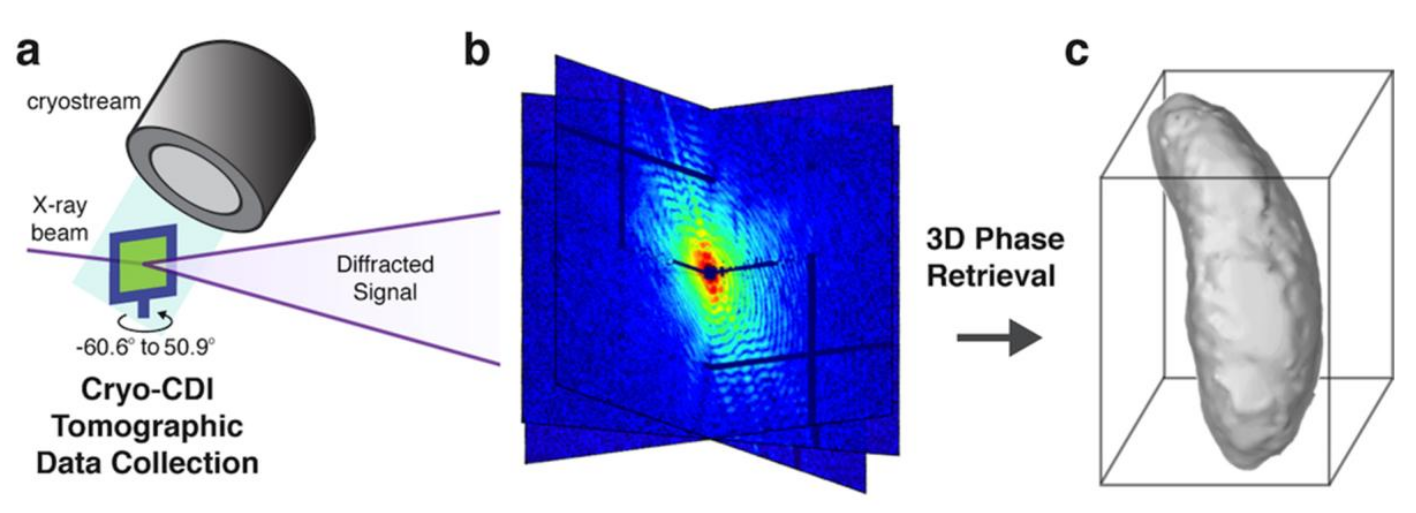
\includegraphics[width=0.5\textwidth]{image.png}
% 	\caption{Three-dimensional reconstruction of a whole, frozen-hydrated N. caninum cell using cryogenic coherent diffraction imaging.
% 	}
% \end{figure}


% \section{Conclusion}

\newpage

\begin{thebibliography}{9}

	\bibitem{Rodriguez}
	Jose A. Rodriguez, Rui Xu, Chien-Chun Chen et al. \emph{Three-dimensional coherent X-ray diffraction imaging of a whole, frozen-hydrated cell} 
	
	\bibitem{2}
	Yoo Jung Kim, Michael P. Fitzgerald et al. \emph{Coherent Imaging with Photonic Lasers} (arXiv Feb 2024)
	\bibitem{}
	Benedikt J.Daurer, \emph{Algorithms for Coherent Diffractive Imaging with X-ray Lasers}, Uppsala Universitet, Uppsala, Sweden.
	
	\bibitem{}
	Chien-Chun Chen, Chun Zu, et al. \emph{Three-dimensional imaging of dislocations in a nanoparticle at atomic resolution} (Nature 2013)
	
	\bibitem{}
	Wenge Yang, Xiaojing Huang, Ross Harder et al. - Coherent diffraction imaging of nonoscale strain evolution in a single crystal under high pressure. (Nature Communications 2012)
	
	\bibitem{}
	Jesse N. Clark, Johannes Ihli, et al. Three-dimensional imaging of dislocation propagation during crystal growth and dislocation. (Nature Materials 2015)
	
	\bibitem{}
	Prosekov et al. \emph{Methods of Coherent X-Ray Diffraction Imaging} (Springer Link 2021)
	
	\bibitem{}
	Chapman et al. \emph{High-reolution ab initio three-dimensional x-ray diffraction microscopy} (Optical Society of America 2006)
	
	\end{thebibliography}
\newpage
% \thispagestyle{lastpage}
\section*{Work Distribution in Group:}
\begin{center}
\fbox{
\begin{minipage}{0.8\textwidth}
\begin{itemize}
	\vspace*{10pt}
	\item \textbf{Pandit Siddhesh Ashok:} Introduction, Types of Coherent Imaging, Methods of CDI specifically CXDI. And typing the document in \LaTeX.code is available at  \\
	\item \textbf{Sujay Hansda:} Three-dimensional coherent X-ray diffraction imaging of a whole, frozen-hydrated cell\\
	\item \textbf{Tarushri N S:} 3D imaging of dislocations in a nanoparticle at atomic resolution, Three-dimensional imaging of dislocation propagation during crystal growth and dissolution, Coherent diffraction imaging of nanoscale strain evolution in a single crystal under high pressure.\\
	\item \textbf{Yogendra Singh Laikara:} Conclusion, Algorithms and Maths behind it.\\
\end{itemize}
\end{minipage}
}
\end{center}
\end{document}